\documentclass[14px]{article}
\usepackage{xeCJK}
\usepackage[frenchb]{babel}
\usepackage[T1]{fontenc}
\usepackage[utf8]{inputenc}
\usepackage{textcomp}
\usepackage{amssymb}
\usepackage[ruled,longend]{algorithm2e}
\usepackage{amsmath}
\usepackage{latexsym}
\usepackage{fancyhdr}
\usepackage{geometry}
\usepackage{setspace}
\usepackage[colorlinks,linkcolor=blue]{hyperref}
% Image
\usepackage{graphicx}
\usepackage{float}
\usepackage{subfigure}
\usepackage{enumerate}


%All LaTeX documents have a ``preamble'' that includes the packages and macros needed to make the document compile. The file `PomonaLgcsFormatting.tex' includes the preamble for this template. You can see it in the file list on the left frame of your screen, and this document is instructed to use it with the \input{} command below.

%\input{PomonaLgcsFormatting}

\begin{document}

\setlength{\parindent}{0pt}
\begin{titlepage}
	\begin{center}
		% Upper part of the page
		
\includegraphics[width=0.35\textwidth]{logo.png}\\[1cm]
		\textsc{\Large Rapport de PSTL}\\[0.5cm]
		% Title
		{ \huge \bfseries Trac-Simulateur \& IDE génériques pour OMicrob}\\[0.4cm]
		% Author and supervisor
		\begin{minipage}{0.4\textwidth}
			\begin{flushleft} \large
				\emph{Author:}\\
				Qiwei \textsc{XIAN}\\
				Ruiwen \textsc{WANG}\\
			\end{flushleft}
		\end{minipage}
		\begin{minipage}{0.4\textwidth}
			\begin{flushright} \large
				\emph{Professeur:} \\
				Prof.\textsc{Emmanuel Chailloux}
			\end{flushright}
		\end{minipage}
		\vfill
		% Bottom of the page
		{\large \today}
	\end{center}

\end{titlepage}
\clearpage

\tableofcontents
\thispagestyle{empty}
\clearpage

\pagestyle{fancy}
\lhead{Introduction}
\rhead{\thepage}
\fancyfoot{}


\section{Introduction}

lien vers les codes sources:
\url{https://github.com/XIANQw/OMicroB/tree/microbit}\\


La programmation des architectures à base de microcontrôleurs est difficile tant par les ressources limitées accessibles que par les modèles de programmation proposés. L'intégration électronique poussée d'un micro-contrôleur permet de diminuer la taille, la consommation électrique et le coût de ces circuits. La taille des programmes et la quantité de mémoire vive sont "faibles", le tas peut être de quelques kilo-octets seulement. Ils doivent communiquer directement avec les dispositifs d'entrées/sorties (capteurs, effecteurs, ...) via les pattes du circuit principal, et ne possèdent pas les périphériques classiques (souris, clavier, écran). La mise au point d'un programme devient plus difficile de par ce manque d'interaction classique.\\

On s'intéresse ici à une nouvelle version portable de la machinerie OCaml, appelée OMicroB, qui engendre un programme C contenant la version byte-code du programme OCaml ainsi que l'interprète de ce byte-code OCaml. Omicrob vient avec un environnement de développement incluant un simulateur permettant de décrire un montage et d'exécuter le programme sur l'ordinateur hôte avant de le transférer sur le microcontrôleur. Bien que portable, la version initiale de l'environnement de développement dont le simulateur a été principalement testée pour l'architecture Arduino. Le portage d'OMicrob vers d'autres architectures (Micro:bit Arm Corex-M0, PIC32) nécessite maintenant d'adapter son environnement de développement, principalement le simulateur. L'idée est d'ajouter une couche d'abstraction aux circuits utilisés pour pouvoir facilement passer d'un microcontrôleur à un autre. Par ailleurs une extension synchrone à flots de données, appelée OCaLustre, est particulièrement appropriée pour décrire les interactions externes et la concurrence interne à l'application. Le couple OCaLustre+OMicroB permet une programmation mixte (synchrone et multi-paradigme classique) avec une consommation parcimonieuse des ressources. L'intérêt de ces couches d'abstractions est de faciliter le développement d'applications fiables sur micro-contrôleurs\\

Ce projet cherche à améliorer cette mise au point de programmes en utilisant d'une part un langage de haut niveau, ici OCaml et son extension synchrone OCaLustre, et d'autre part en fournissant un simulateur et un IDE simple pour la mise au point de tels programmes.

\clearpage
\pagestyle{fancy}
\lhead{Structure de compilation}
\rhead{\thepage}
\fancyfoot{}

\section{Structure de compilation}
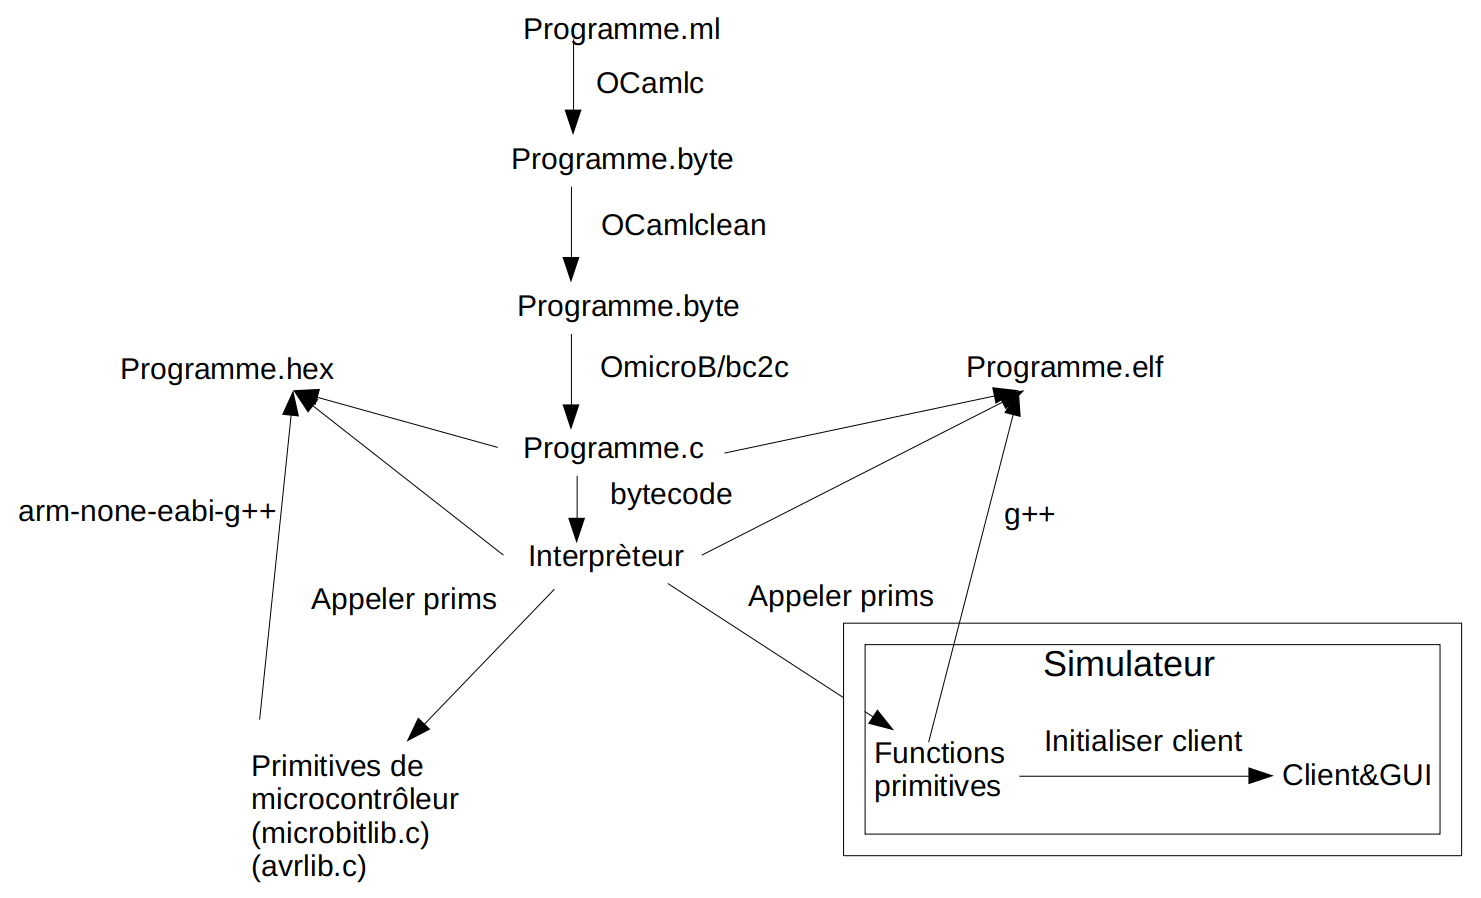
\includegraphics[width=\textwidth]{StructureProgramme.png}\\[1cm]
Cet image montre chaque étape de compilation d'un programme OCaml par OMicroB.
\begin{enumerate}
	\item \textbf{ocamlc} compile le fichier \textbf{.ml} avec la bibliothèque et génére un fichier \textbf{.byte}.
	\item \textbf{ocamlclean} traite le fichier généré \textbf{.byte}.
	\item \textbf{bc2c} est le compilateur de \textbf{OMicroB}, il permet de transférer le code binaire à un programme \textbf{.c}.
	\item \textbf{g++} compile le \textbf{programme.c} et la bibliothèque de simulateur \textbf{sf-regs} puis génère le fichier exécutable \textbf{.elf}.
	\item \textbf{arm-none-eabi-g++} compile le \textbf{programme.c} avec la bibliothèque de microcontrôleur (avrlib, microbitlib, etc) puis génére le fichier exécutable \textbf{.hex}.\\
\end{enumerate}

\textbf{OMicroB} produit deux fichiers exécutables après de compiler un programme \textbf{OCaml}.

- \textbf{.elf} est exécutable en mode simulation, il permet de démarrer le simulateur et montrer le changement des états de pin et les effets de programme sur une interface graphique.\\
- \textbf{.hex} est exécutable sur un microcontrôleur.

\clearpage
\pagestyle{fancy}
\lhead{Composition du simulateur}
\rhead{\thepage}
\fancyfoot{}
\section{Composition du simulateur}
Le simulatuer est composé du coté de client et du coté de serveur, ainsi que un langage de description pour le montage des périphériques sur un microcontrôleur.

\subsection{Montage}
Pour démarrer le processus client et implémenter l'interface graphique, le client a besoin de savoir quels composants du microcontrôleur il doit visualiser sur l'interface graphique. Donc
nous devons proposer un fichier \textbf{circuit.txt} qui décrit les composants du microcontrôleur et les associations entre chaque composant et les Pins correspondants. Avant de démarrer le processus client, le processus analyse est exécuté pour évaluer ce fichier. Une structure qui contient ces informations est stockée dans un mémoire partagé après l'évaluation. Le client peut recevoir les informations des composants du microcontrôleur depuis ce mémoire partagé.\\
Cette fonctionnalité est réalisée dans le dossier \textbf{src/byterun/montage}, la structure est définie dans \textbf{src/byterun/simul/share.h}.

\subsection{Client}
La partie client est programmée par C dans \textbf{src/byterun/client}, se compose de deux fichiers.
\begin{enumerate}
\item \textbf{client.c} définit les fonctions du travail par exemple traiter le message qui vient du côté server.

\item \textbf{gui.c} implémente l'interface graphique par \textbf{gtk3.0}.
il nous montre un UI de simulateur permet de visualiser le résultat de programme et les états des Pins pendant la simulation, ainsi que l'interaction par les boutons.\\
\end{enumerate}

\subsection{Serveur}
La partie serveur est codée par C dans "/src/byterun/", il contient des fichiers:
\begin{enumerate}
\item \textbf{/src/byterun/vm}.
Ce dossier contient les fichiers de l'interprèteur d'OMicroB, par exemple le format des type basiques de données, le gc de machine virtuelle ainsi que les définition des instructions de code binaire. Il exécute le programme OCaml et envoie les instructions des codes binaires au serveur.

\item \textbf{/src/byterun/simul/sf-regs.c/.h}.
C'est la bibliothèque des primitives de simulateur, lorsque le programme utilise un primitive par exemple \textbf{set\_pin}, l'interprèteur va appeler le primitive correspondant dans la bibliothèque, le serveur envoie l'instruction au côté client après le calcul.

\item \textbf{src/byterun/shared.c/.h}.
Ce fichier définit des structures de données partagées
entre le processus client et serveur, elles sont stockées dans un mémoire partagé au fur et mesure de l'exécution de programme.
\end{enumerate}


\clearpage
\pagestyle{fancy}
\lhead{Architecture du simulateur}
\rhead{\thepage}
\fancyfoot{}
\section{Architecture du simulateur}
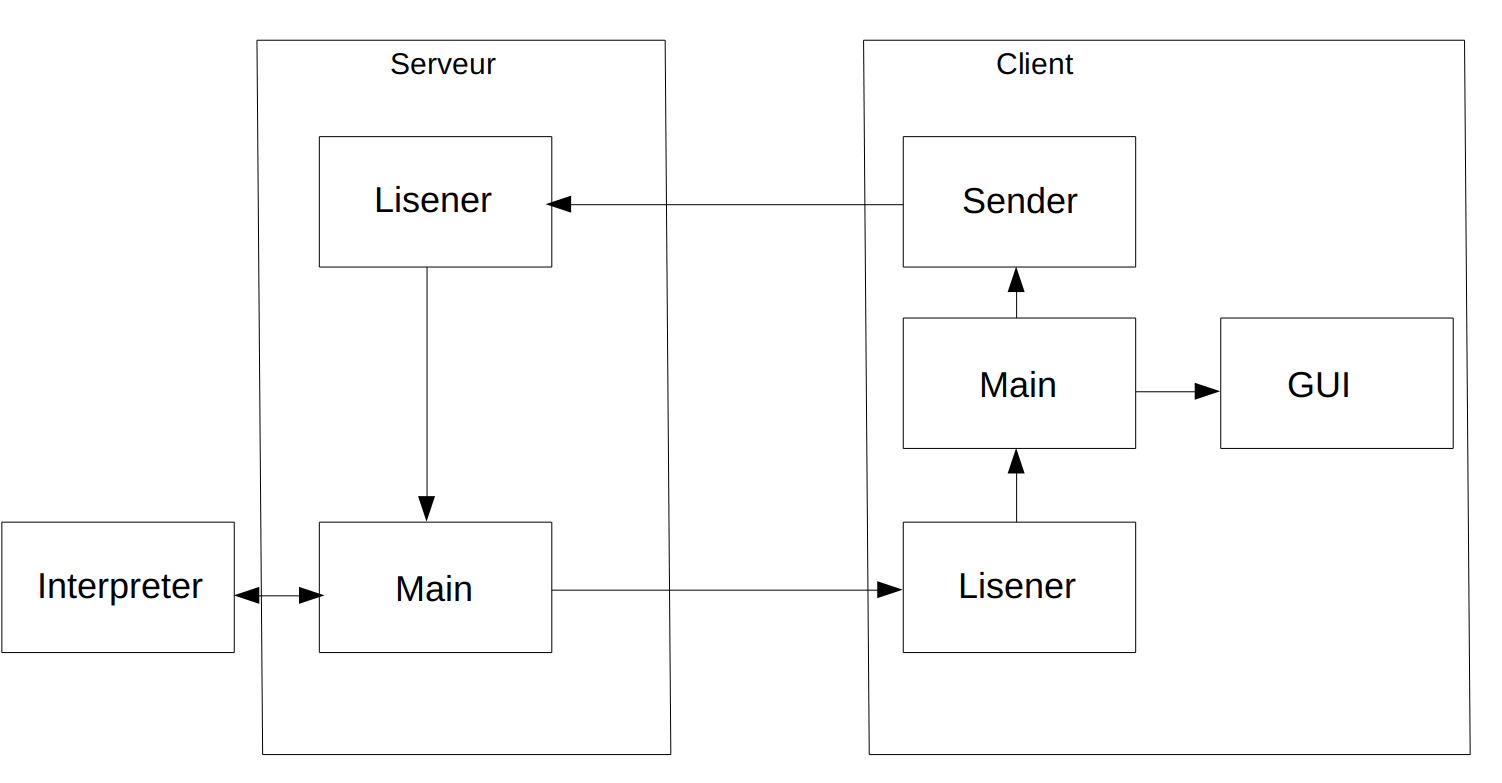
\includegraphics[width=\textwidth]{simulator.png}\\[1cm]
Cet image décrit globalement la structure du simulateur. On l'a réalisé par \textbf{l'architecture serveur-client} et il exécute deux processus en concurrence. Chaque processus exécute plusieurs threads et travaille asynchroniquement.\\

\subsection{Tâche du thread}
\textbf{Processus Serveur} exécute deux threads, \textbf{lisener} et \textbf{Main}.
\begin{enumerate}
	\item \textbf{Main} traite simplement l'instruction qui vient de l'interprèteur et envoyer au thread \textbf{lisener} de client.
	\item \textbf{lisener} reçoit l'instruction venant de \textbf{Sender} et informer \textbf{Main}.
\end{enumerate}

\textbf{Processus Client} tourne simultanément quatre threads, \textbf{Main}, \textbf{GUI}, \textbf{Sender} et \textbf{Lisener}.
\begin{enumerate}
	\item \textbf{Main} est le premier thread principal, il traite les arguments venant de processus serveur et connecte aux mémoires partagés, par exemple le mémoire partagé pour la communication et pour le montage. Il est responsable d'exécuter les autres threads.
	\item \textbf{GUI} crée les composants de l'interface graphique en fonction de l'information du montage. Il actualise l'interface dans un boucle infini afin de visualiser le changement des états de chaque composant simultanément.
	\item \textbf{Sender} sert à traiter input de l'utilisateur et envoyer l'instruction au serveur, par exemple appuyer les boutons.
	\item \textbf{Lisener} reçoit l'instruction venant de serveur, en plus manipuler les composants de l'interface graphique en fonction de l'instruction.
\end{enumerate}

\clearpage

\subsection{Mécanisem de communication}
La mémoire partagée sert à communiquer entre le serveur et client, puisque c'est la plus rapide manière du transport de données. Mais son inconvénient est que l'on doit implémenter un mécanisme de synchronization afin de protéger les données partagées pour la lecture et l'écriture. Donc pour deux directions du transport (du serveur au client et du client au serveur), on a besoin de deux mémoires partagées, \textbf{shm1} est écrit par le serveur, le client le lit. \textbf{shm2} est inversé.\\

Afin de synchroniser la lecture et l'écriture, on met un mutex et une variable conditionnelle pour chaque mémoire partagée. Il garant que chaque instruction de serveur peut être bien traiter.\\

\textbf{Sénario du traitement d'une instruction}
\begin{enumerate}
	\item \textbf{client lisener} se bloque pour attendre l'instruction de serveur.
	\item \textbf{serveur main} demande le mutex
	\item \textbf{serveur main} vérifie la variable conditionnelle.\\
	- Si la condition se satisfait, il passe à l'étape suivant.
	- Sinon, cela veut dire que l'instruction dernière n'est pas encore traitée par client, \textbf{serveur main} se bloque.
	\item \textbf{serveur main} envoie l'instruction au client.
	\item \textbf{serveur main} débloque le thread \textbf{client lisener}.
	\item \textbf{serveur main} rend le mutex.
	\item \textbf{client lisener} est débloqué, demande le mutex.
	\item \textbf{client lisener} vérifie si la condition se satisfait.
	- Si oui, cela veut dire que la nouvelle instruction arrive, il passe à l'étape suivant.
	- Sinon, c'est un déblocage fausse, il se bloque.
	\item \textbf{client lisener} informe au \textbf{GUI} afin de visualiser le nouvel état de composant.
	\item \textbf{client lisener} débloque le thread \textbf{serveur main}.
	\item \textbf{client lisener} rend le mutex.
	\item retour à l'étape 1.
\end{enumerate}

\clearpage

\subsection{Protocole}
Le protocole est un rôle de transférer les informations entre coté client et coté serveur. Il est un entier de 32 bits. la structure est (numéro de méthode 7bits) :: arguments(25 bits).
Afin de représenter le protocole en un entier de 32 bits. on a utilisé 7 bits pour le nom de fonction, alors on peut étendre jusqu'à 128 primitives maximum. \\
(S -> C) indique que la direction de l'envoie est du serveur au client.

\begin{enumerate}
\item[-] \textbf{SET\_PIXEL(x,y,val)}: 1(7bits)::x(12 bits)::y(12 bits)::val(1 bits)\\
(S -> C) Modifier l'état du pixel des coordonnées x et y à val.\\
Dans la version de haut niveau, ce protocole sert à modifier directement l'état de pixel. Dans la version de bas niveau, ce protocole est remplacé par SET\_PIN.

\item[-] \textbf{CLEAN\_SCREEN}: 2(32 bits)\\
(S -> C) Mettre les états de tous les pixels à 0, envoyé par \textbf{microbit\_clean\_screen}.

\item[-] \textbf{SET\_PIN(p,n)}: 3(7 bits)::p(8 bits)::n(17 bits)\\
(S -> C) Modifier le pin p au niveau n. (n = 0 ou 1), envoyé par \textbf{microbit\_digital\_write}.

\item[-] \textbf{WRITE\_PIN(p,v)}: 4(7 bits)::p(8 bits)::v(17 bits)\\
(S -> C) Modifier le pin p à la valeur v (0 <= v <= 1024), envoyé par \textbf{microbit\_analog\_write}.

\item[-] \textbf{APPUIE\_A}: 0(32 bits)\\
(C -> S) Inverser l'état du bouton A.

\item[-] \textbf{APPUIE\_B}: 1(32 bits)\\
(C -> S) Inverser l'état du bouton B.
\end{enumerate}

\clearpage

\section{Fonctionalités Implémentées}
\subsection{Visualiser les phrases sur la matrice des leds}
Tout d'abord,nous convertissons les informations de chaque caractère en forme des graphiques raster dans une table en code hexadécimal 5x8 bits en bien tirer par order du code ASCII.Lorsqu'on recevoir un command d'imprimer une caractère à l'écran,
on va calculer ASCII code correspond à cette caractère,et puis en fonction de ce ASCII code ,on peut calculer le décalage dans la table de code hexadécimal correspond à cette caractère. Sortir enfin les 5 * 8 bits d'information dont il dispose. Prendre 5 * 5 bits d'entre eux et les imprimer pixel par pixel sur l'écran.\\

Une exemple de visualiser la caractère 'A' sur la matrice des leds.
\begin{enumerate}
	\item calcule le code ASCII de 'A', c'est 65.
	\item calcule son décalage c'est 65 * 5 = 325.(parce que l'écran est de 5 lignes et chaque ligne est composé de 2 chiffre hexadécimal)
	\item cherche son table de code hexadécimal correspondant dans le tableau, c'est \{30,28,38,28,28\}.
	\item nous convertissons code hexadécimal en forme code binaire.\\
	00110000\\
	00101000\\
	00111000\\
	00101000\\
	00101000\\
	\item modifier les Pins de chaque LED en fonction de cette code binaire. On a finalement une image comme cela.\\
	\centering
	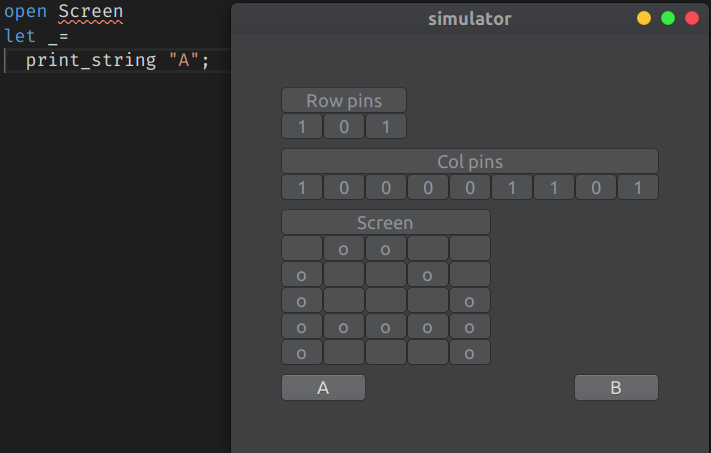
\includegraphics[width=0.6\textwidth]{printA.png}\\[1cm]

\end{enumerate}

\clearpage

\subsection{Analyser le ficher du montage}
Pour le montage de microcontrôleur, il a besoin d'un fichier qui stocke les informations de chaque composant de microcontrôleur comme le nombre des pins, les association entre chaque composant et le pin correspondant. Une fois que le simulateur connait ces informations, il peut implémenter l'interface graphique et contrôler les composants par modifier l'état des pins.\\
Donc on a utilisé Flex, Yacc et langage C afin de réaliser un langage descriptif.
\begin{enumerate}
	\item On défini les \textbf{tokens} dans le fichier \textbf{parser.y}.
	\item Lier les mots prédéfinis avec ces tokens dans \textbf{lexer.lex}
	\item Créer les noeuds de \textbf{AST}(l'arbre d'analyse syntaxe) dans fichier \textbf{AST.c} et \textbf{AST.h}.
	\item Réaliser les fonctions de l'évaluation dans le fichier \textbf{get\_env.c}.
\end{enumerate}

\begin{figure}[htbp]
	\subfigure[cf.exmple \textbf{circuit.txt}]{
		\begin{minipage}[t]{\linewidth}
			\centering
			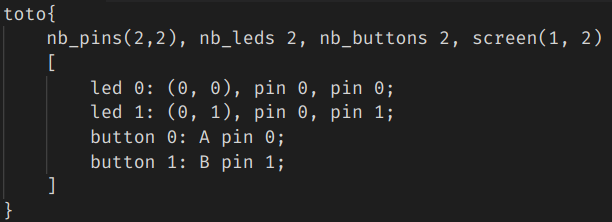
\includegraphics[width=0.5\textwidth]{circuit_ex.png}\\[1cm]
			%\caption{fig1}
		\end{minipage}%
	}%
\end{figure}

\textbf{Le grammaire et les mots prédéfinis}
\begin{enumerate}
	\item \textbf{nom du simulateur\{l'information du montage\}}: C'est la structure du langage.
	\item \textbf{nb\_pins (num\_row, num\_col)}: \textbf{num\_row} est le nombre de pins de ligne(row), \textbf{num\_col} est celui de colonne.
	\item \textbf{nb\_leds num}: \textbf{num} est le nombre de leds.
	\item \textbf{nb\_buttons num}: \textbf{num} est le nombre de buttons.
	\item \textbf{screen(row, col)}: Cela indique le nombre de ligne et colonne de matrice des LEDs.
	\item \textbf{led id: (row, col), pin id1, pin id2}: Cela représente le numéro du LED et ses coordonnées dans la matrice, ainsi que l'association entre le led et deux pins correspondant. id1 est l'identifiant de pin row, id2 est celui de pin col.
	\item \textbf{button id: étiquette pin id}: Cette une déclaration du bouton dont l'identifiant est id et son étiquette, ainsi que le pin correspondant.
\end{enumerate}

\clearpage
\pagestyle{fancy}
\lhead{Méthodologie de réalisation}
\rhead{\thepage}
\fancyfoot{}

\clearpage

\section{Méthodologie de réalisation}
Selon ce qui précède, notre objectif est de simuler les informations d'entrée et de sortie du micro-controlleur monopuce, pour réaliser les fonctionnalité du simulateur, il y a deux versions, en \textbf{haut niveau} et en \textbf{bas niveau}.

\subsection{Version haut niveau}
\textbf{haut niveau} est que l'on simule abstraitement un microcontrôleur, on implémente les tableau pour stocker les états de chaque composant. Dès que l'état de composant est modifier par le primitive, on modifie le tableau directement.\\
Par exemple le serveur appelle le primitive \textbf{microbit\_write\_pixel 0 0 true}, il a juste besoin de modifier le tableau qui stock l'état des LEDs. pixels[0][0] = true.\\

\textbf{Avantage}\\
La version est plus simple, il a juste besoin de modifier le tableau correspondant.\\

\textbf{Inconvénient}\\
Cette méthode n'est pas généralle, parce que les composants sont différents pour les microcontôleurs divers, on ne peut pas implémenter les tableau pour chaque microcontrôleur.

\subsection{Version bas niveau}
\textbf{bas niveau} est que l'on simule réellement un microcontrôleur, afin de mieux simuler l'état de fonctionnement réel du microcontrôleur à partir de l'architecture du microcontrôleur, nous espérons modifier directement l'état du \textbf{tableau de pins}, sans avoir besoin d'autres appels de fonctions, et refléter directement les effets de ces modifications sur \textbf{l'interface graphique}. Cela fera quelques changements basés sur le haut niveau précédent.

Par exemple, Un \textbf{LED} est contrôlé par deux \textbf{pins}(\textbf{pin\_row} et \textbf{pin\_col}) dans le circuit du microcontrôleur réel. Lorsque nous voulons allumer un led, nous devons d'abord chercher son \textbf{pin\_row} et \textbf{pin\_col} correspondant, puis mettons \textbf{pin\_row} à haut niveau et \textbf{pin\_col} à bas niveau.\\

\textbf{Avantage}
Cette version est générale pour tous les microcontrôleurs, parce que on manipule directement les états de \textbf{pins} au lieu de composant. Même si le microcontrôleur est changé, on a juste besoin de changer un fichier du montage, mais pas le simulateur.\\

\textbf{Inconvénient}
Le traitement d'une instruction est plus compliqué, l'interaction entre le serveur et le client est plus fréquente. Par exemple, pour allumer un \textbf{LED}, le serveur envoie une seule instruction \textbf{SET\_PIXEL(X,Y,True)} au client dans la version haut niveau. Mais dans le bas niveau, le serveur doit d'abord chercher le \textbf{pin\_row} et \textbf{pin\_col}, puis envoyer deux instructions \textbf{SET\_PIN(pin\_row, 1)} et \textbf{SET\_PIN(pin\_col, 0)} au client.

\clearpage

\section{Sénarios et Tests}
Ce sont les étapes de simuler un programme ocaml par la simulateur du microbit.
\begin{enumerate}
	\item Charger l'information du montage par un fichier \textbf{circuit.txt}.
	\item Le processus montage analyse ce fichier et génère une structure du montage, en plus envoie au serveur et au client par le mémoire partagée \textbf{envid}.
	\item Le processus client implémente une interface graphique en fonction de structure du montage.
	\begin{figure}[htbp]
		\centering
		\subfigure[la description du circuit]{
			\begin{minipage}[t]{0.4\linewidth}
				\centering
				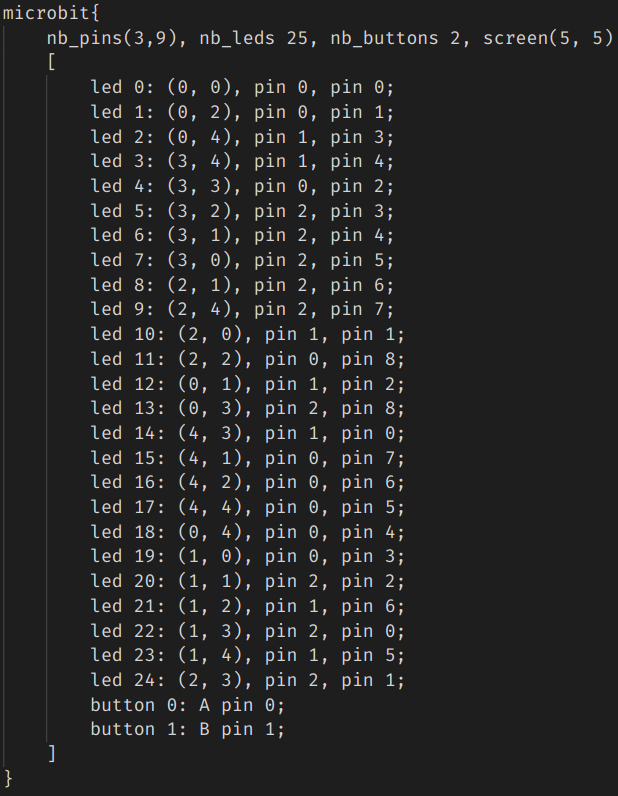
\includegraphics[width=\textwidth]{circuit.png}
			\end{minipage}%
		}%
		\subfigure[l'interface graphique de microbit]{
			\begin{minipage}[t]{0.4\linewidth}
				\centering
				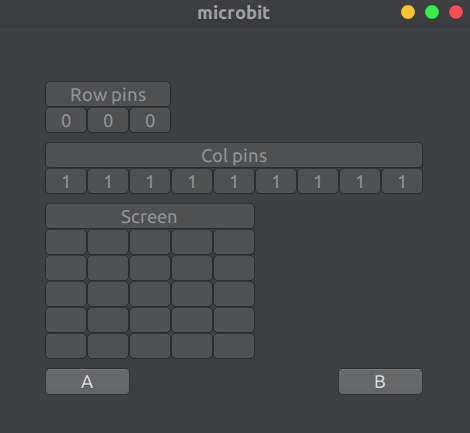
\includegraphics[width=\textwidth]{gui.png}
			\end{minipage}%
		}%
		\centering
	\end{figure}
	\item Le serveur interprète le programme OCaml, puis envoie des protocoles au client.
	\item Le client visualise les effets du programme.
	\begin{figure}[htbp]
		\centering
		\subfigure[un programme ocaml]{
			\begin{minipage}[t]{0.3\linewidth}
				\centering
				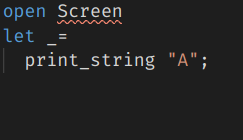
\includegraphics[width=\textwidth]{printAprog.png}
			\end{minipage}%
		}%
		\subfigure[L'effet de la visualisation]{
			\begin{minipage}[t]{0.3\linewidth}
				\centering
				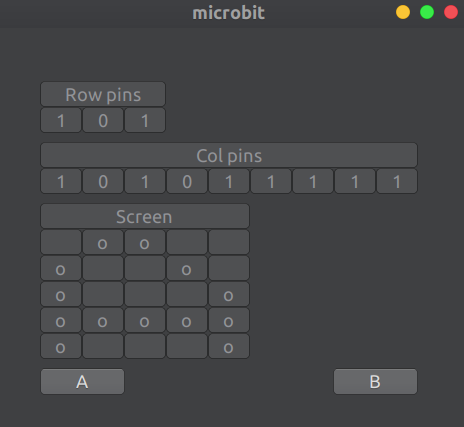
\includegraphics[width=\textwidth]{printAeffets.png}
			\end{minipage}%
		}%
		\centering
	\end{figure}

\end{enumerate}
\clearpage

\section{Problème et Solution}
\subsection{Choix de processus ou de thread}
Quand on désigne l'architecture du simulateur, on a deux choix pour le côté du serveur et client. Soit on les sépare en deux threads, soit deux processus. Les avantages du thread est que c'est plus facile de partager les données et réaliser la synchronization. Néanmoins, la partie serveur est compilé par \textbf{ocamlc} dans une étape de la compilation, et nous utilisons \textbf{gtk+3.0} pour réaliser l'interface graphique, le compilateur \textbf{ocamlc} ne peut pas compiler la bibliothèque de \textbf{gtk+3.0}, donc on sépare le serveur et le client en deux processus.


\subsection{Synchronization}
Comme ce que l'on a présenté, le serveur envoie les protocoles au client, et le client visualise simultanément les états de chaque composant, mais pour quelque protocole par exemple \textbf{CLEARSCREEN}, il prend du temps parce qu'il faut éteindre tous les LEDs. Donc s'il n'y a pas de mécanisme de synchronization afin de garantir que le nouveau protocole arrive après le traitement du protocole précédent, il risque de perdre quelques instructions.

Pour synchroniser le transfert du protocole entre le serveur et le client, nous avons essayé plusieurs méthodes diverses dans le processus du développement.


\subsubsection{Pipe + Signal}
Au début, nous utilisions le pipe et le signal pour transmettre le protocole. Pour la direction du serveur au client, le protocole est transmis par le pipe, et la direction inverse, on a utilisé le signal pour représenter le protocole, parce qu'il n'y a que deux protocoles(\textbf{APPUIE\_A} et \textbf{APPUIE\_B}). Le serveur traite le protocole par la fonction \textbf{handler}.
Son avantage est que l'on n'a plus besoin exécuter un thread \textbf{lisener} dans le processus \textbf{serveur}. Comme la fonction \textbf{handler} exécute dès que le processus serveur reçoit le sigal depuis le processus client. \\
Mais la mécanisme de signal est très limité, le signal utilisable est divers pour le système différent, par exemple pour linux on a droit d'utiliser les signaux qui sont supérieur à 32, mais pour macOS, il y a seulement quatres signaux qu'on peut utiliser.

\subsubsection{Pipe}
Après qu'on a constaté la limite du signal, on a essayé d'utiliser deux pipes pour la communication en deux direction. Pipe possède la mécanisme de protection, et il peut  synchroniser automatiquement la communication, mais il génère un fichier temporaire pour la lecture et l'écriture, ainsi que il est moins efficace que la mémoire partagée. Donc on a finalement décidé d'utiliser la mémoire partagée.

\clearpage

\subsection{Problème de conflit}
\begin{figure}[htbp]
	\subfigure[cf.le circuit réel de microbit]{
		\begin{minipage}[t]{\linewidth}
			\centering
			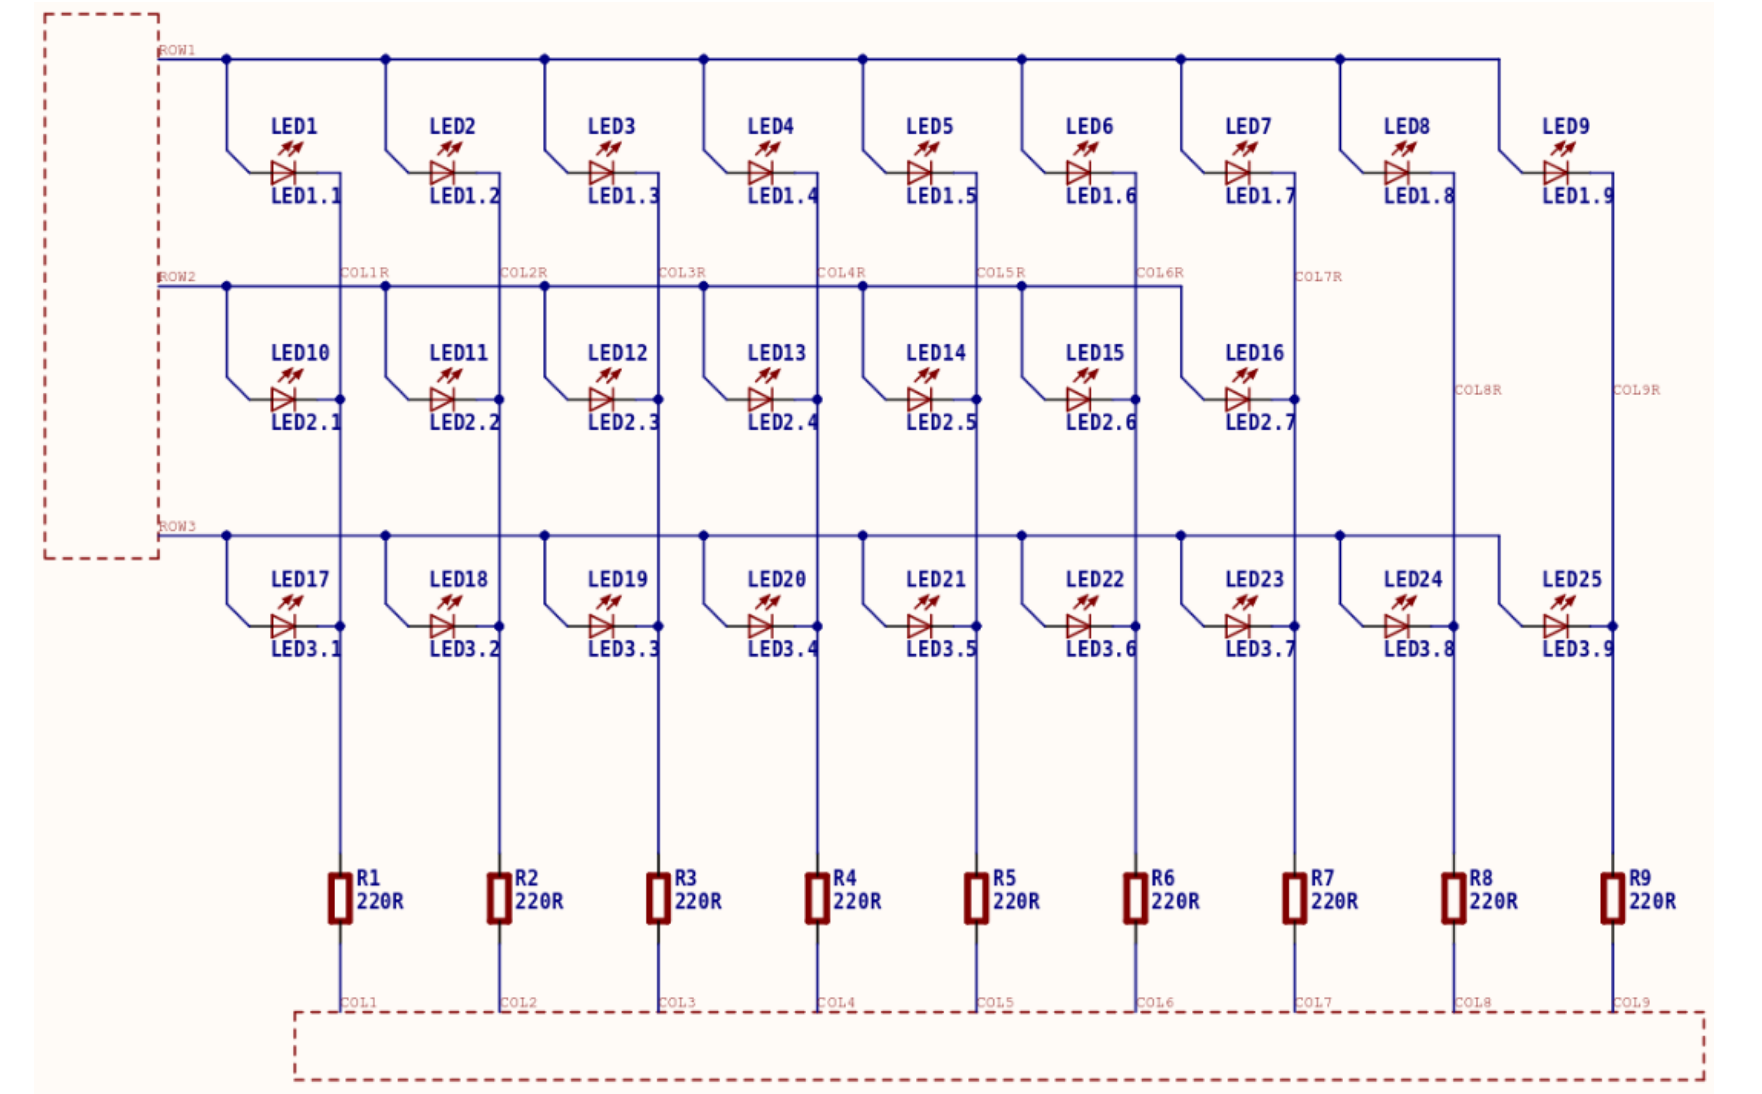
\includegraphics[width=0.8\textwidth]{circuitReelMicrobit.png}
		\end{minipage}%
	}%
\end{figure}
Cet image montre le circuit du \textbf{microbit}, la matrice de LED se compose d'une matrice de pins de 3 * 9. Pour allumer un LED, on doit mettre le \textbf{pin\_row} correspondant au niveau \textbf{HIGH}, et mettre son \textbf{pin\_col} au niveau \textbf{LOW}.

\begin{figure}[htbp]
	\subfigure[cf.le tableau des associations entre le LED et les pins correspondant]{
		\begin{minipage}[t]{\linewidth}
			\centering
			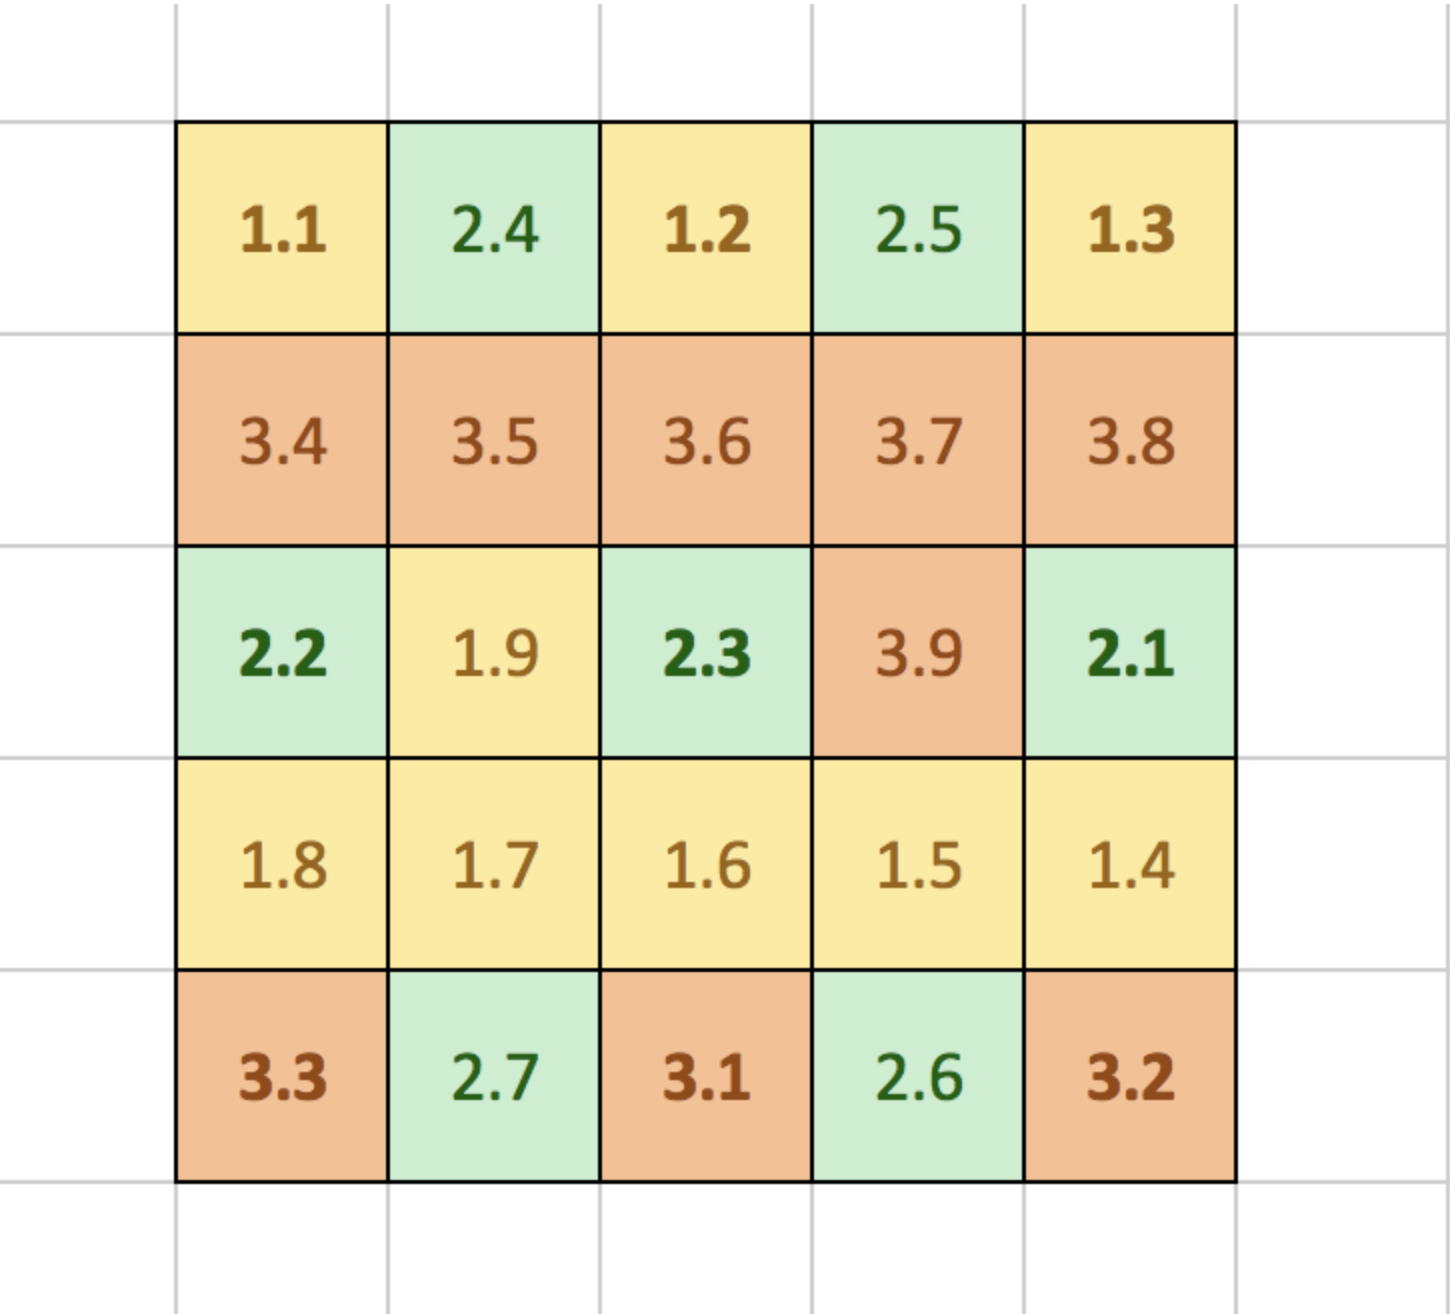
\includegraphics[width=0.3\textwidth]{matrice_Pins.png}
			%\caption{fig1}
		\end{minipage}%
	}%
\end{figure}
Ce tableau montre la relation de position entre le circuit du  \textbf{microbit} et l'éran du \textbf{microbit}.
\clearpage
Lorsque nous voulons allumer un seulement LED, il n'y a pas de conflit. Par exemple, pour \textbf{LED 0 0}, on met \textbf{pin\_row1} au niveau \textbf{HIGH}, et \textbf{pin\_col1} au niveau \textbf{LOW}. Les effets de la simulation est comme cet image.\\
\begin{figure}[htbp]
	\subfigure[cf.exmple \textbf{allumer LED 0 0}]{
		\begin{minipage}[t]{\linewidth}
			\centering
			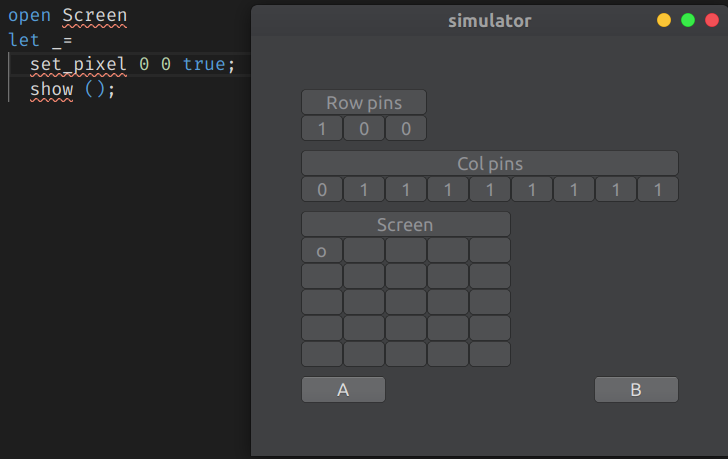
\includegraphics[width=0.5\textwidth]{no-conflict.png}\\[1cm]
			%\caption{fig1}
		\end{minipage}%
	}%
\end{figure}\\

Néanmoins, si on veut allumer deux LEDs dont le pin\_row n'est pas la même, il y aura le conflit. Par exemple on allume \textbf{LED 0 0} et \textbf{LED 0 1}. On doit mettre \textbf{pin\_row1} et \textbf{pin\_row3} au niveau \textbf{HIGH}, mettre \textbf{pin\_col1} et \textbf{pin\_col4} au niveau \textbf{LOW}. Dans ce cas-là, il y aura quatre LEDs allumé.
\begin{enumerate}
	\item \textbf{LED 0 0} correspondant à \textbf{pin\_row1, pin\_col1}.
	\item \textbf{LED 4 3} correspondant à \textbf{pin\_row1, pin\_col4}.
	\item \textbf{LED 0 1} correspondant à \textbf{pin\_row3, pin\_col4}.
	\item \textbf{LED 2 4} correspondant à \textbf{pin\_row3, pin\_col1}.
\end{enumerate}
\begin{figure}[htbp]
	\subfigure[cf.exmple \textbf{allumer LED 0 0 et LED 0 1}]{
		\begin{minipage}[t]{\linewidth}
			\centering
			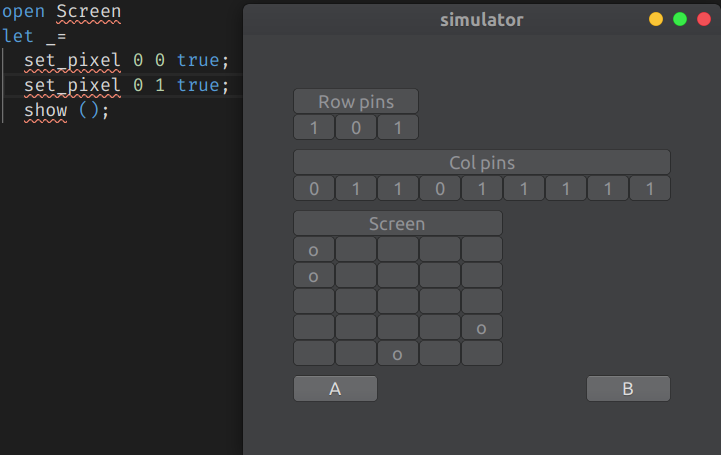
\includegraphics[width=0.5\textwidth]{conflit.png}\\[1cm]
			%\caption{fig1}
		\end{minipage}%
	}%
\end{figure}



\end{document}
